%--------------------------------------------------------------------%
% REV01: Fri 23 Jul 2021 20:08:29 WIB (RMS)
% Berkas utama templat LaTeX.
% author Petra Barus, Peb Ruswono Aryan
%--------------------------------------------------------------------%
% Berkas ini berisi struktur utama dokumen LaTeX yang akan dibuat.
%--------------------------------------------------------------------%
\documentclass[12pt, a4paper, onecolumn, oneside, final]{report}

%-------------------------------------------------------------------%
%
% Konfigurasi dokumen LaTeX untuk laporan tesis IF ITB
%
% @author Petra Novandi
%
%-------------------------------------------------------------------%
%
% Berkas asli berasal dari Steven Lolong
%
%-------------------------------------------------------------------%

% Ukuran kertas
\special{papersize=210mm,297mm}

% Setting margin
\usepackage[top=3cm,bottom=2.5cm,left=4cm,right=2.5cm]{geometry}

\usepackage{mathptmx}

% Judul bahasa Indonesia
\usepackage[bahasa]{babel}

% Format citation
%\usepackage[backend=bibtex,citestyle=authoryear]{biblatex}
\usepackage{natbib}

\usepackage[utf8]{inputenc}
\usepackage{microtype}
\usepackage{makecell}
\usepackage{graphicx}
\usepackage{csquotes}
\usepackage{tabularx}
\usepackage{listings}
\usepackage{tabto}
\usepackage{comment}
\usepackage{amsmath}
\usepackage[labelfont=bf]{caption}
\usepackage{enumitem}
\usepackage{tocbibind}
\usepackage{tocloft}
\usepackage{float}
\usepackage{indentfirst}
\usepackage[auto]{chappg}
\usepackage{titling}
\usepackage{blindtext}
\usepackage{sectsty}
\usepackage{chngcntr}
\usepackage{etoolbox}
\usepackage{hyperref}  
\usepackage{titlesec}
\usepackage{parskip}
\usepackage[htt]{hyphenat}
\usepackage{longtable}
\usepackage{pgfgantt}
\usepackage{booktabs}
\usepackage{pifont}
\usepackage{siunitx}
\usepackage[section]{placeins}
\usepackage{algorithm}
\usepackage{algpseudocode}
 
% \usepackage{ragged2e}
% \usepackage{libertine}
% \usepackage{array}
% \usepackage{textcase}
% \usepackage{setspace}
% \usepackage{afterpage}

% Line satu setengah spasi
\renewcommand{\baselinestretch}{1.5}

% Setting judul
\titlespacing*{\chapter}{0pt}{-50pt}{10pt}
\chapterfont{\centering \Large}
\titleformat{\chapter}[display]
  {\Large\centering\bfseries}
  {\chaptertitlename\ \thechapter}{0pt}
    {\Large\bfseries\uppercase}

% Setting nomor pada subbsubsubbab
\setcounter{secnumdepth}{3}
\setcounter{tocdepth}{4}

\makeatletter
\setlength{\@fptop}{0pt}
\setlength{\@fpbot}{0pt plus 1fil}
\makeatother

% Counter untuk figure dan table.
\counterwithin{figure}{chapter}
\counterwithin{table}{chapter}

% Counter untuk penomoran halaman lanjut
\newcounter{savepage}

% Kode lebih kecil
% \let\OldTexttt\texttt
% \renewcommand{\texttt}[1]{\OldTexttt{\footnotesize{#1}}}

% Pengaturan Caption
\captionsetup{labelsep=space}

% Pengaturan spasi untuk justify
\pretolerance=10000
\tolerance=2000 
\emergencystretch=10pt
%\tolerance=1
%\emergencystretch=10pt
%\hyphenpenalty=10000
%\exhyphenpenalty=1000

% Pengaturan untuk Daftar Rumus
\newcommand{\listequationsname}{Daftar Rumus}
\newlistof{myequations}{equ}{\listequationsname}
\newcommand{\myequations}[1]{%
\addcontentsline{equ}{myequations}{\protect\numberline{\theequation}#1}\par}
\setlength{\cftmyequationsnumwidth}{2.5em}

%\newcommand{\listalgorithmname}{Daftar Algoritme}
%\newlistof{algorithm}{alg}{\listalgorithmname}
%\newcommand{\algorithm}[1]{%
%\refstepcounter{algorithm}
%\par\noindent\centering\normalsize\textbf{Algoritme {\thechapter.\thealgorithm\ }\normalfont #1}
%\addcontentsline{alg}{algorithm}{\protect\numberline{\thechapter.\thealgorithm}#1}\par}
%\setlength{\cftalgorithmnumwidth}{2.5em}

% Pengaturan untuk title Daftar Isi, Tabel, dan Gambar
\renewcommand{\cfttoctitlefont}{\hspace*{\fill}\Large\bfseries\MakeUppercase}
\renewcommand{\cftaftertoctitle}{\hspace*{\fill}}
\renewcommand{\cftlottitlefont}{\hspace*{\fill}\Large\bfseries\MakeUppercase}
\renewcommand{\cftafterlottitle}{\hspace*{\fill}}
\renewcommand{\cftloftitlefont}{\hspace*{\fill}\Large\bfseries\MakeUppercase}
\renewcommand{\cftafterloftitle}{\hspace*{\fill}} 
\renewcommand{\cftequtitlefont}{\hspace*{\fill}\Large\bfseries\MakeUppercase}
\renewcommand{\cftafterequtitle}{\hspace*{\fill}} 
%\renewcommand{\cftalgtitlefont}{\hspace*{\fill}\Large\bfseries\MakeUppercase}
%\renewcommand{\cftafteralgtitle}{\hspace*{\fill}} 

\renewcommand{\cftchappresnum}{Bab }
\renewcommand{\cftchapaftersnum}{}
\renewcommand{\cftchapnumwidth}{3.7em}

\setlength{\cftbeforetoctitleskip}{-4em}
\setlength{\cftbeforeloftitleskip}{-4em}
\setlength{\cftbeforelottitleskip}{-4em}
\setlength{\cftbeforeequtitleskip}{-4em}
%\setlength{\cftbeforealgtitleskip}{-4em}

\newcolumntype{Y}{>{\centering\arraybackslash}X}

% Listing Code thingy
\lstset{frame=single,
  columns=fullflexible,
  basicstyle={\small\ttfamily},
  breaklines=true,
  breakatwhitespace=false,
  postbreak=\mbox{$\hookrightarrow$\space},
  tabsize=3
}
\renewcommand{\lstlistingname}{Kode}
\renewcommand{\lstlistlistingname}{Daftar \lstlistingname}
% \newcommand{\listingsfont}{\ttfamily}
% https://en.wikibooks.org/wiki/LaTeX/Source_Code_Listings
\renewcommand{\cftchapleader}{\cftdotfill{\cftdotsep}}

\cftsetpnumwidth{2em}


% \DefineBibliographyStrings{english}{%
%     urlseen = {Waktu akses},
%     url = {URL:},
%     and = {dan},
%     andothers = {dkk\adddot},
%     in = {dalam}
% }

% Add comma between Author and Year
%\renewcommand*{\nameyeardelim}{\addcomma\space}

% \titleformat{\paragraph}
% {\normalfont\normalsize\bfseries}{\theparagraph}{1em}{}
% \titlespacing*{\paragraph}
% {0pt}{3.25ex plus 1ex minus .2ex}{1.5ex plus .2ex}

% \titlespacing*{\section} {0pt}{2.5ex plus 1ex minus .2ex}{1.3ex plus .2ex}
% \titlespacing*{\subsection} {0pt}{2.25ex plus 1ex minus .2ex}{0.5ex plus .2ex}

% For Gantt Chart
% \newcounter{myWeekNum}
% \stepcounter{myWeekNum}
% 
% \newcommand{\myWeek}{\themyWeekNum
%     \stepcounter{myWeekNum}
%     \ifnum\themyWeekNum=53
%          \setcounter{myWeekNum}{1}
%     \else\fi
% }
% 
% \newcolumntype{L}[1]{>{\raggedright\let\newline\\\arraybackslash\hspace{0pt}}m{#1}}
% \newcolumntype{C}[1]{>{\centering\let\newline\\\arraybackslash\hspace{0pt}}m{#1}}
% \newcolumntype{R}[1]{>{\raggedleft\let\newline\\\arraybackslash\hspace{0pt}}m{#1}}
%
% \makeatletter
% \def\@chapter[#1]#2{\ifnum \c@secnumdepth >\m@ne
%                          \refstepcounter{chapter}%
%                          \typeout{\@chapapp\space\thechapter.}%
%                          \addcontentsline{toc}{chapter}%
%                                    {\protect{BAB \numberline{\thechapter}\texorpdfstring{\uppercase{#1}}{#1}}}%
%                     \else
%                       \addcontentsline{toc}{chapter}{\texorpdfstring{\uppercase{#1}}{#1}}%
%                     \fi
%                     \chaptermark{#1}%
%                     \addtocontents{lof}{\protect\addvspace{10\p@}}%
%                     \addtocontents{lot}{\protect\addvspace{10\p@}}%
%                     \if@twocolumn
%                       \@topnewpage[\@makechapterhead{#2}]%
%                     \else
%                       \@makechapterhead{#2}%
%                       \@afterheading
%                     \fi}
% \makeatother


\makeatletter

\makeatother
%\bibliography{references}
\begin{document}

%Basic configuration
\title{Pengembangan Sistem Tracing untuk mendukung pelacakan Request Causality antar Service dalam Arsitektur Microservice}
\date{27 Oktober}
\newcommand{\yearsidang}{2021}
\newcommand{\jenislaporan}{Draf Bab 3 Tugas Akhir}
\author{Rafi Abbel Mohammad}
\newcommand{\nim}{182180272}

\pagenumbering{roman}
\setcounter{page}{0}

\clearpage
\pagestyle{empty}

\begin{center}
    \smallskip

    \Large \MakeUppercase{\bfseries \thetitle}
    \vfill

    \normalsize \MakeUppercase{Laporan \jenislaporan}
    \vfill

    \normalsize Disusun sebagai syarat kelulusan tingkat sarjana
    \vfill

    \normalsize oleh:

    \normalsize \theauthor \\
    \normalsize NIM: \nim

    \vfill
    \begin{figure}[h]
        \centering
        
\includegraphics[width=0.25\textwidth]{resources/cover-ganesha.jpg}
    \end{figure}
    \vfill

    \large
    \uppercase{
        Program Studi Sistem dan Teknologi Informasi \\
        Sekolah Teknik Elektro dan Informatika \\
        Institut Teknologi Bandung
    }

    \yearsidang

\end{center}

\clearpage

\clearpage
\pagestyle{empty}

\begin{center}
    \smallskip

    \Large \bfseries \MakeUppercase{\thetitle}
    \vfill

    \Large Laporan Tugas Akhir
    \vfill

    \large Oleh

    \Large \theauthor

    \large Program Studi Teknik Informatika \\
    \normalsize \normalfont
    Sekolah Teknik Elektro dan Informatika \\
    Institut Teknologi Bandung \\

    \vfill
    \normalsize \normalfont
    Telah disetujui dan disahkan sebagai Laporan Tugas Akhir \\ di Bandung, 23 Agustus 2017 \\
    Mengetahui,

    \vfill
    \setlength{\tabcolsep}{12pt}
    \begin{tabularx}{\textwidth}{c@{\hskip 0.2\textwidth}cc@{\hskip 0.3\textwidth}}
         & {\bfseries Pembimbing}                                   & \\
         &                                                          & \\
         &                                                          & \\
         &                                                          & \\
         &                                                          & \\
         & \underline{Dr. I Gusti Bagus Baskara Nugraha S.T., M.T.} & \\
         & NIP. 19760124 201012 1 001                               &
    \end{tabularx}

\end{center}
\clearpage


\pagestyle{plain}


\titleformat*{\section}{\centering\bfseries\Large\MakeUpperCase}

\clearpage
\tableofcontents

\clearpage
{%
    \let\oldnumberline\numberline%
    \renewcommand{\numberline}{\figurename~\oldnumberline}%
    \listoffigures%
}

\clearpage
{%
    \let\oldnumberline\numberline%
    \renewcommand{\numberline}{\tablename~\oldnumberline}%
    \listoftables%
}

\clearpage
{%
    \let\oldnumberline\numberline%
    \renewcommand{\numberline}{\lstlistingname~\oldnumberline}%
    \lstlistoflistings%
}

\newpage
\setcounter{savepage}{\arabic{page}}

\titleformat*{\section}{\bfseries\large}

%----------------------------------------------------------------%
% Konfigurasi Bab
%----------------------------------------------------------------%
\renewcommand{\chaptername}{BAB}
\renewcommand{\thechapter}{\Roman{chapter}}
\pagenumbering{bychapter}
\setlength{\parindent}{1cm}
%----------------------------------------------------------------%

%----------------------------------------------------------------%
% Dafter Bab
% Untuk menambahkan daftar bab, buat berkas bab misalnya `chapter-6` di direktori `chapters`, dan masukkan ke sini.
%----------------------------------------------------------------%
\chapter{Pendahuluan}

Pada bab ini akan dibahas mengenai gambaran dasar dari pelaksanaan Tugas Akhir dalam bentuk penjelasan latar belakang yang mendasari pemilihan topik. Dari latar belakang tersebut, akan diurai kembali menjadi rumusan masalah, tujuan, batasan masalah, serta metodologi yang digunakan untuk keperluan Tugas Akhir ini.

\section{Latar Belakang}

Aplikasi \textit{spreadsheet} merupakan aplikasi yang mudah ditemui dan wajar digunakan oleh banyak orang, baik secara personal maupun dalam sebuah organisasi komersial \citep{Chan1996}. Pada tahun 1979, aplikasi \textit{spreadsheet} pertama dibuat dengan nama VisiCalc. Pengguna komputer pada saat itu dimanjakan dengan kapabilitas dan fleksibilitas aplikasi yang dapat melakukan operasi sederhana tanpa harus menggunakan komputer \textit{mainframe}. Dengan semakin berkembangnya daya komputasi, saat ini telah banyak sekali muncul aplikasi \textit{spreadsheet} baru dan penggunaannya juga semakin beragam.

\textit{Spreadsheet} iliki beberapa keunggulan dibandingkan dengan aplikasi pengolahan data jenis lain. Keunggulan yang paling terlihat adalah banyak orang yang mengetahui cara penggunaan aplikasi jenis \textit{spreadsheet} dan terbiasa dalam menggunakannya. Di samping itu, \textit{spreadsheet} memiliki banyak fitur dan kemampuan yang jarang diketahui orang awam jika digunakan dengan benar. Dengan keunggulan ini, \textit{spreadsheet} sering kali dijadikan pilihan utama dalam pengolahan dan pengumpulan data. Beberapa orang mungkin menganggap, penggunaan \textit{spreadsheet} adalah personal sehingga tidak membutuhkan tim atau bantuan orang lain dalam pembuatan suatu \textit{spreadsheet}. Hal ini tidak dapat dibenarkan, karena jika melihat kasus penggunaannya pada organisasi bisnis yang besar, \textit{spreadsheet} yang dihasilkan sangatlah kompleks dan besar dengan pengembangan yang membutuhkan banyak orang \citep{Panko1998}.

Penggunaan \textit{spreadsheet} yang dapat ditemui pada perusahaan atau instansi adalah sebagai media pengumpulan data. Data yang dikumpulkan biasanya dalam bentuk \textit{data frame} yakni \textit{spreadsheet} yang mempunyai dua struktur utama yaitu bagian \textit{value} atau data dan bagian \textit{atribute} atau label \citep{Chen2013}. Data yang telah dikumpulkan biasanya akan disebarkan kepada pihak-pihak yang membutuhkan atau disimpan sebagai arsip data yang akan digunakan kembali pada saat dibutuhkan.

Sebagai media pengumpulan data, \textit{spreadsheet} memiliki permasalahan penyimpanan data. Hal tersebut penting untuk diperhatikan jika data yang dikumpulkan mungkin tidak hanya akan ditampilkan dalam bentuk \textit{spreadsheet} namun juga dapat digunakan oleh aplikasi lain. Permasalahan lain yang mungkin muncul adalah kompleksitas dan besarnya ukuran data pada \textit{spreadsheet} yang membuat penggunaan \textit{spreadsheet} pada sebuah bisnis sangatlah rentan akan kesalahan. Sebuah kesalahan kecil dapat berakibat fatal dan memberikan kerugian seperti kehilangan pendapatan, kesalahan pemberian harga, penipuan, dan kegagalan sistem akibat ketergantungan berlebih antar \textit{spreadsheet} \citep{EUSPRIGAbout}. Telah banyak bukti dan penelitian yang menunjukan bahwa kesalahan pada \textit{spreadsheet} sangat mudah ditemui. %Bahkan pada \textit{spreadsheet} yang dibuat dengan sangat hati-hati, masih dapat ditemui sekitar 1 persen atau lebih kesalahan pada formula yang dibuat \citep{Panko1998}.
Contoh kesalahan yang dapat terjadi adalah kesalahan tipe data, kesalahan masukan, tidak divalidasinya data masukan, serta permasalahan \textit{single version of truth} dimana bisa terdapat dua atau lebih versi dari data yang sama.

% Tingginya angka kesalahan yang dapat terjadi pada suatu \textit{spreadsheet} merupakan hal yang sangat krusial terutama di dalam bisnis. Metode pencegahan harus dapat dilakukan untuk dapat mengurangi angka kesalahan ini. Beberapa organisasi dapat menerapkan pencegahan dengan cara melakukan tahap-tahap metodologi yakni dengan pembuatan desain awal, melakukan metode \textit{best practice} yang tersedia dan sesuai dengan situasi yang dihadapi, menerapkan \textit{policy} khusus pada saat pembuatan \textit{spreadsheet}, melakukan \textit{testing}, serta pembuatan dokumentasi \citep{EUSPRIGBestPractice}. Namun, metodologi tersebut masih sangat rentan oleh kesalahan manusia karena perangkat lunak yang digunakan tetap tidak diubah didalam menjalankan metodologi tersebut.

Untuk dapat mengurangi kesalahan-kesalahan yang sering terjadi pada \textit{spreadsheet} secara lebih mendasar, dibutuhkan bantuan perangkat lunak untuk dapat melakukan kontrol terhadap masukan pengguna, melakukan validasi, serta dapat melakukan penyimpanan data yang telah dikumpulkan. Pada tugas akhir ini akan difokuskan pada pengembangan sebuah aplikasi pengumpulan data berbentuk \textit{spreadsheet} yang dapat membantu pengguna mengurangi terjadinya masalah-masalah yang telah disebutkan sebelumnya.

\section{Rumusan Masalah}\label{RumusanMasalah}

Seperti yang telah dijelaskan pada latar belakang, salah satu penggunaan aplikasi \textit{spreadsheet} adalah sebagai media pengumpulan data. Beberapa permasalahan yang muncul dalam pengumpulan data adalah kolaborasi, validasi, dan penyimpanan data. Pengumpulan data dapat dilakukan oleh banyak orang secara bersama-sama sehingga dapat menyebabkan konflik pada data masukan. Konflik ini bisa terjadi karena terdapat lebih dari satu versi file yang diubah secara bersama-sama. Di samping itu, data yang dimasukkan biasanya tidak melalui proses validasi sehingga dapat menyalahi domain data yang seharusnya. Setelah data dikumpulkan ke dalam bentuk \textit{spreadsheet}, diperlukan media penyimpanan data sehingga data tidak terisolasi. Contoh dari media penyimpanan tersebut adalah menggunakan basis data.

Hal-hal tersebut merupakan beberapa masalah utama yang cukup penting untuk diselesaikan terutama dalam penggunaannya pada bisnis dan komersial sehingga akan dibentuk sebuah kakas yang membantu pengumpulan data pada format \textit{spreadsheet}. Dalam rangka pembangunan kakas, terdapat beberapa permasalahan yang menjadi perhatian pada tugas akhir ini, yaitu:

\begin{enumerate}
    %\item Bagaimana cara menangani konflik yang terjadi pada saat kolaborasi?
    \item Bagaimana cara melakukan validasi terhadap data masukan?
    \item Bagaimana cara data pada \textit{spreadsheet} dapat disimpan pada basis data?
    \item Bagaimana cara melakukan penyimpanan data yang telah dibuat?
    \item Bagaimana proposal perubahan alur kerja yang terjadi akibat penggunaan kakas yang dibuat?
\end{enumerate}

\section{Tujuan}

Tujuan yang ingin dicapai dalam Tugas Akhir ini adalah mengembangkan perangkat lunak pengumpulan data berbentuk \textit{spreadsheet} yang dapat mengubah data dalam format \textit{spreadsheet} menjadi data relasional serta melakukan validasi pada data masukan. Dengan adanya perangkat lunak ini diharapkan dapat dilakukan pengumpulan data yang disertai validasi data masukan.

\section{Batasan Masalah}

Dalam pengerjaan Tugas Akhir ini, terdapat beberapa batasan-batasan yang perlu diperhatikan. Batasan tersebut ditujukan untuk memperjelas dan memfokuskan objek penelitian dan pengembangan tugas akhir. Batasan-batasan masalah pengerjaan tugas akhir adalah sebagai berikut,

\begin{enumerate}
    %\item Fitur kolaborasi pada \textit{spreadsheet} bukan fokus utama, fitur akan diambil dari aplikasi \textit{spreadsheet} yang telah ada.
    %\item Fokus data masukan pada Tugas Akhir ini berupa data mentah yang belum direkapitulasi.
    \item Kakas hanya dapat berjalan pada aplikasi EtherCalc.
    \item Jenis \textit{spreadsheet} yang ditangani adalah \textit{data frame} dan relasi.
    \item Data disimpan dalam bentuk basis data relasional.
    \item Basis data yang didukung untuk digunakan dalam penyimpanan data hanya MySQL.
    \item Struktur basis data dan tingkat normalisasi yang terbentuk merupakan tanggung jawab pengguna dan tidak ditangani oleh kakas.
    \item Kakas hanya mendukung penggunaan satu \textit{sheet} dalam satu \textit{spreadsheet}.
    \item Validasi yang dilakukan hanya validasi tipe, domain, dan relasi data.
    \item Validasi tipe hanya mencakup tipe \textit{integer}, \textit{double}, \textit{string}, dan \textit{boolean}.
    \item Validasi domain hanya mencakup aturan \textit{range}, lebih besar, lebih kecil, sama dengan, dan nilai diskrit. Atribut hanya dapat menerima satu aturan validasi domain.
\end{enumerate}

\section{Metodologi}

Metodologi yang digunakan dalam pengerjaan Tugas Akhir ini yakni:
\begin{enumerate}
    \item Studi Literatur \\
          Pengerjaan tugas akhir diawali dengan mencari dan mempelajari referensi berupa jurnal ilmiah dan aplikasi-aplikasi yang telah ada sebelumnya yang dapat membantu pengembangan kakas yang dibuat pada tugas akhir ini. Literatur yang dicari dan dipelajari berkaitan dengan topik tugas akhir yaitu mengenai \textit{spreadsheet}, penggunaannya pada bisnis, kesalahan yang sering dilakukan dalam pembuatan, teknik pendeteksian data yang ada pada \textit{spreadsheet}, serta hal-hal lain yang masih berkaitan dengan topik tugas akhir ini.

    \item Analisis Masalah \\
          Pada tahap ini dilakukan analisis permasalahan yang berkaitan dengan topik yang diangkat pada tugas akhir ini. Diantaranya adalah memecah permasalahan menjadi aplikasi \textit{spreadsheet} yang dikembangkan, penanganan konflik saat berkolaborasi, jenis \textit{spreadsheet} yang ditangani, metode interaksi pengguna, penentuan bagian data dan label, representasi tabel, validasi data, penyimpanan data, interaksi antar \textit{spreadsheet}, dan proposal perubahan alur kerja.

    \item Perancangan Solusi \\
          Pada tahap ini dilakukan perancangan solusi yang dapat menyelesaikan masalah-masalah yang telah dijelaskan pada bagian analisis masalah. Bagian perancangan ini juga menjelaskan arsitektur yang digunakan untuk membangun perangkat lunak berdasarkan spesifikasi dan metode yang digunakan.

    \item Implementasi \\
          Pada tahap ini dilakukan pembangunan kakas sesuai dengan kebutuhan dan spesifikasi dari hasil analisis masalah serta rancangan solusi yang diajukan.

    \item Pengujian dan Analisis Hasil \\
          Pada tahap ini dilakukan pengujian dengan menggunakan data set uji yang sesuai dengan batasan masalah ke dalam kakas yang diimplementasikan. Selanjutnya dilakukan analisis hasil pengujian dan penarikan kesimpulan.

\end{enumerate}

\section{Sistematika Pembahasan}

Penulisan tugas akhir ini terdiri dari 5 bab, yaitu: BAB I Pendahuluan, BAB II Tinjauan Pustaka, BAB III Analisis dan Perancangan, BAB IV Rancangan, Implementasi, dan Pengujian, dan BAB V Penutup.

Bab satu membahas mengenai latar belakang permasalahan, rumusan masalah, tujuan, batasan masalah, metodologi serta sistematika pembahasan yang digunakan. Bab ini juga menjelaskan secara umum isi dari tugas besar serta gambaran dasar dari pelaksanaan tugas akhir.

Bab dua menjelaskan mengenai dasar teori yang digunakan di dalam menyelesaikan permasalahan yang diangkat. Teori yang digunakan berasal dari literatur dan referensi yang berhubungan dengan permasalahan yang diangkat seperti hal-hal yang berkaitan dengan \textit{spreadsheet}, penggunaannya pada bisnis, masalah yang sering terjadi dalam pembuatan, metode \textit{quality control} yang dapat dilakukan untuk mencegah kesalahan, serta metode pendeteksian bagian label dan data yang pernah dibuat pada penelitian lain. Dasar teori ini menjadi dasar analisis dan rancangan solusi pada bab selanjutnya.

Bab tiga memaparkan analisa kebutuhan dan permasalahan yang dipilih yakni tingginya tingkat kesalahan yang terjadi pada \textit{spreadsheet}. Dari hasil analisa yang dilakukan, di dapatkan bentuk solusi umum yang dapat digunakan untuk mengatasi permasalahan tersebut. Selanjutnya solusi umum tersebut dibuat rancangan dan arsitekturnya agar dapat diimplementasikan.

Bab empat memperlihatkan rancangan perangkat lunak yang dibuat serta hasil implementasinya. Pada akhir bab akan ditunjukkan hasil pengujian yang dilakukan kepada kakas yang dibuat dan pembahasan dari pengujian tersebut. Pengujian dilakukan untuk mengetahui keberhasilan kakas yang dibuat untuk menyelesaikan permasalahan yang di definisikan pada rumusan masalah.

Bab lima berisikan kesimpulan terhadap hasil implementasi dan solusi yang dipaparkan untuk menyelesaikan permasalahan. Di samping itu, terdapat bagian saran yang memaparkan saran pengembangan dan perbaikan yang dapat dilakukan untuk memperkaya fitur dan menyelesaikan permasalahan yang lebih luas.

% \section{Jadwal Pelaksanaan}
% \newsavebox\mybox
% \begin{lrbox}{\mybox}
%     \begin{ganttchart}[
%     vgrid={*{6}{draw=none}, dotted},
%     x unit=.05cm,
%     y unit title=.6cm,
%     y unit chart=.6cm,
%     time slot format=isodate,
%     time slot format/start date=2016-09-01]{2016-09-01}{2017-04-30}
%     \ganttset{bar height=.6}
%     \gantttitlecalendar{year, month} \\
%     \ganttbar[bar/.append style={fill=blue}]{Tahap 1}{2016-09-01}{2016-11-30}\\
%     \ganttbar[bar/.append style={fill=blue}]{Tahap 2}{2016-10-01}{2016-11-15}\\
%     \ganttbar[bar/.append style={fill=blue}]{Tahap 3}{2016-11-01}{2016-12-15}\\
%     \ganttbar[bar/.append style={fill=blue}]{Tahap 4}{2016-12-15}{2017-03-01}\\
%     \ganttbar[bar/.append style={fill=blue}]{Tahap 5}{2017-02-01}{2017-04-30}
%     \end{ganttchart}
% \end{lrbox}

% Pengerjaan tugas akhir ini direncanakan mulai pada September 2016 sampai April 2016. Pelaksanaan tugas akhir ini dibagi menjadi 5 tahap yang dapat dipetakan kepada metodologi pengerjaan sebagai berikut,
% \begin{enumerate}
%     \item Tahap 1: Studi Literatur
%     \item Tahap 2: Analisis Masalah
%     \item Tahap 3: Perancangan Solusi
%     \item Tahap 4: Implementasi
%     \item Tahap 5: Pengujian dan Analisis Hasil
% \end{enumerate}
% Jadwal pelaksanaan tugas akhir berdasarkan metodologi pengerjaan tugas akhir dapat dilihat pada Tabel \ref{Gantt-Chart} dibawah ini.
% \begin{table}[htb]
% \centering
% \caption{Gantt Chart jadwal pelaksanaan tugas akhir}
% \label{Gantt-Chart}
% \tikz{
%   \node[inner sep=0pt,outer sep=0pt] (gantt)
%   {\begin{tabular}{c}
%     \toprule
%     \resizebox{\textwidth}{!}{\usebox\mybox} \\
%     \bottomrule
%    \end{tabular}%
%    };
% }   
% \end{table}
\chapter{Studi Literatur}

Bab ini akan berisi pembahasan dari studi literatur yang akan berkaitan dengan permasalahan yang dibahas di Tugas Akhir ini. Hasil studi literatur akan menjadi dasar dalam pengerjaan Tugas Akhir ini baik untuk menganalisis masalah dan juga untuk merancang solusi.

\section{Distributed Tracing}
\label{bab2-dtracing}

\subsection{\textit{Overview} Distributed Tracing}
Dengan meningkatnya penggunaan Microservice, cara untuk melakukan \textit{profiling}, \textit{debugging}, dan \textit{monitoring} aplikasi menjadi berbeda dengan cara yang dilakukan pada aplikasi yang berbentuk Monolith.
Salah satu cara untuk melakukan profiling pada aplikasi berbasis Microservice adalah dengan Distributed Tracing.
Distributed Tracing, disebut juga dengan Distributed Request Tracing, adalah sebuah tipe logging terkorelasi yang dapat memberikan pengguna mendapatkan visibilitas pada operasi dari perangkat lunak terdistribusi untuk kasus seperti debugging di environment \textit{production}, dan analisis penggalian akar masalah pada kegagalan atau insiden lainnya \citep{parker2020distributed}.
Dengan adanya kakas Distributed Tracing, pengguna dapat mendapatkan insight mengenai operasi yang terjadi di aplikasi terdistribusi secara kolektif dengan cara melakukan pelacakan pada \textit{request} yang dibuat oleh suatu \textit{service}.

Kita bisa sebut setiap pekerjaan yang dilakukan oleh sebuah \textit{service} dalam suatu waktu sebagai \textit{span}.
Setiap \textit{span} bisa diisi dengan \textit{metadata}, seringkali disebut sebagai \textit{attributes} atau \textit{tags}, dan \textit{events}, seringkali disebut sebagai \textit{logs}.
Setiap pemanggilan Remote Procedure Call (RPC) atau Application Programming Interface (API) antara \textit{service} akan merepresentasikan hubungan dari \textit{request} yang terjadi diantara \textit{service} tersebut.
Hubungan tersebut disebarkan diantara \textit{service} sebagai \textit{trace context}, yaitu data yang secara unik mendefinisikan \textit{span} yang dibuat oleh setiap \textit{service}.
Setiap \textit{span} yang dibuat oleh setiap \textit{service} tersebut diteruskan kepada proses eksternal yang dapat dikumpulkan atau diagregasi sebagai sebuah \textit{trace}.
\textit{Trace} tersebut dapat dianalisis lebih lanjut dan disimpan untuk mendapatkan \textit{insight} mengenai \textit{service}.
Berikut adalah ilustrasi sederhana mengenai \textit{trace}:
\begin{figure}[htb]
      \centering
      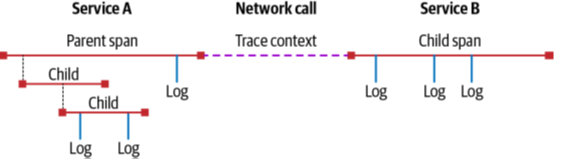
\includegraphics[width=1\textwidth]{resources/ch2/tracing-illus.png}
      \caption{Ilustrasi Tracing}
      \label{TracingIlllustration}
\end{figure}

Adapun komponen-komponen yang membangun sistem Distributed Tracing adalah sebagai berikut \citep{parker2020distributed}:
\begin{enumerate}
      \item Instrumentasi \\
            Distributed Tracing membutuhkan data \textit{trace} agar dapat bekerja.
            Data \textit{trace} dihasilkan dengan cara menginstrumentasikan proses-proses \textit{service} atau mentrasformasikan data telemetri yang sudah ada ke data \textit{trace}.
      \item \textit{Deployment} \\
            Setelah data \textit{trace} dihasilkan, kita perlu mengirimkan data tersebut ke suatu tempat.
            Melakukan \textit{deployment} pada sistem \textit{tracing} membutuhkan pemahaman dimana perangkat lunak kita dijalankan di \textit{server} dan bagaimana perangkat tersebut dijalankan.
            Agar dapat memaksimalkan kemampuan dari \textit{tracing} juga meminimalkan \textit{overhead} yang terjadi pada aplikasi, kita perlu memahami teknik yang cocok untuk melakukan deployment pada sistem Distributed Tracing yang akan kita gunakan.
      \item Penyampaian \textit{Value} \\
            Saat \textit{service} kita telah dapat menghasilkan data \textit{trace} dan kita telah memiliki infrastruktur yang diperlukan untuk mengolah data \textit{trace} tersebut, kita akan memerlukan kakas yang tepat untuk menggabungkan \textit{trace} dari berbagai \textit{service} dengan metadata lain seperti \textit{metrics} dan \textit{logs} untuk dapat menghasilkan \textit{value} yang berguna bagi proses \textit{debugging}, \textit{profiling}, dan \textit{monitoring} perangkat lunak terdistribusi.
\end{enumerate}

\subsection{\textit{Context Propagation}}

\subsection{\textit{Critical Path}}
\label{crit-path}

%\subsection{Komponen Distributed Tracing}
%
%\subsubsection{Instrumentasi}
%
%\subsubsection{\textit{Deployment}}
%
%\subsubsection{\textit{Value Delivery}}



%\subsection{Pelacakan \textit{request causality}}
%\label{bab2-dtracing-causality}

\section{gRPC}
gRPC adalah sebuah \textit{framework} Remote Procedure Call (RPC) Open Source berperforma tinggi yang dapat dijalankan di berbagai environment \citep{grpc}.
gRPC dapat secara efisien menghubungkan \textit{service} yang berada di dalam dan antara data center dengan berbagai dukungan untuk melakukan load balancing, tracing, pengecekan kesehatan, dan autentikasi.
gRPC juga dapat diaplikasikan pada server yang terdistribusi untuk menghubungkan berbagai perangkat mulai dari aplikasi mobile dan browser ke layanan backend.
Seperti RPC pada umumnya, gRPC memungkinkan \textit{service} yang terpisah untuk mengakses fungsi layaknya objek lokal. Ada beberapa skenario penggunaan utama dari gRPC:
\begin{enumerate}
	\item Menghubungkan service-service yang bersifat poliglot seperti dalam arsitektur Microservice.
	\item Menghubungkan perangkat mobile, browser client ke service backend.
	\item Menghasilkan library bagi sisi client yang efisien.
\end{enumerate}

Secara default, gRPC menggunakan Protocol Buffers sebagai Interface Definition Language (IDL) dan juga sebagai format pertukaran pesannya (walaupun juga bisa menggunakan JSON sebagai format pertukaran data).
Langkah pertama ketika menggunakan Protocol Buffers adalah dengan mendefinisikan struktur dari data yang ingin diserialisasi dalam sebuah file proto, yaitu sebuah file teks biasa yang memiliki ekstensi “.proto”.
Data dari Protocol Buffers distrukturkan sebagai messages yang masing-masing memiliki catatan mengenai data yang berbentuk pasangan name-value yang disebut dengan fields.
Berikut adalah contoh sederhana dari file proto:
\lstinputlisting[captionpos=b, caption={Contoh File Proto}]{codes/ch2/hello.proto}

Ketika struktur data sudah dibuat, kode Proto tersebut perlu di compile menggunakan kakas bernama protoc yang akan membuat akses data dalam bahsa pemrograman yang dipilih.
gRPC menggunakan protoc untuk menghasilkan kode dari file Proto berupa: kode gRPC bagi client dan server, dan juga kode Protocol Buffer biasa yang digunakan untuk melakukan populasi, serialisasi, dan kode untuk mendapatkan tipe pesan.

Adapun penggunaan gRPC pada sistem client dan server adalah sebagai berikut:
\begin{enumerate}
	\item Mendefinisikan service beserta method apa saja yang bisa dipanggil beserta parameter dan juga return type bagi masing-masing method.
	\item  Server akan mengimplementasi interface hasil kompilasi protoc yang berasal dari method-method yang didefinisikan pada file proto.
	\item Client akan memanggil method yang sudah didefinisikan pada server.
\end{enumerate}



%\section{Protokol Komunikasi Microservice}
%Pada subbab ini akan dijelaskan beberapa protokol komunikasi yang bisa digunakan dalam arsitektur Microsevice.
%\subsection{REST API}
%Representational State Transfer (REST) merupakan sebuah gaya arsitektur yang dibuat untuk mendesain sistem yang berjalan di World Wide Web.
%REST pertama kali diperkenalkan oleh Roy Thomas Fielding dalam disertasinya pada tahun 2005 yang berjudul \textit{Architectural Styles and the Design of Network-based Software Architectures}.
%Dalam mendesain arsitektur, REST mendefinisikan beberapa aturan yaitu skalabilitas antara komponen yang berinteraksi, antar muka yang seragam, \textit{deployment} yang independen bagi komponen, dan pembuatan arsitektur berlapis yang dapat memfasilitasi komponen untuk melakukan \textit{caching} agar dapat mengurangi \textit{latency}, memperkuat \textit{security}, dan mengenkapsulasi sistem \textit{legacy} \citep{rest}.
%
%Application Programming Interface (API) yang didesain berdasarkan prinsip-prinsip REST disebut dengan RESTful API.
%Ada dua konsep utama yang dipakai dalam mendesain REST API yaitu \textit{resources}, atau sumber daya, dan \textit{representations}, atau representasi \citep{restful-book}.
%Resource yang dimaksud dalam konteks RESTful API bisa berarti apa saja yang cukup penting untuk direferensi dan diakses sebagai API.
%Sebuah \textit{resource} biasanya sesuatu yang dapat disimpan dalam komputer seperti sebuah data yang disimpan dalam database ataupun sebuah hasil dari eksekusi algoritme.
%Satu-satunya batasan pada setiap \textit{resource} tersebut adalah setiap resource harus memiliki sebuah URL.
%Representasi sendiri menggambarkan bagaimana kondisi atau \textit{\textit{state}} saat \textit{resource} tersebut diakses.
%Contoh paling umum dari representasi  RESTful API adalah mentransportasikan \textit{resource} melalui protokol HTTP dan dalam bentuk data JSON.
%
%Dalam praktiknya, \textit{resource} sendiri tidak bisa diakses dengan sembarang cara.
%Dalam sistem RESTful API, client dan server berinteraksi dengan saling mengirim pesan yang mengikuti protokol yang sudah ditentukan sebelumnya, dalam hal ini adalah mengikuti semantik dari protokol HTTP itu sendiri.
%HTTP mendefinisikan delapan jenis pesan yang berbeda, namun ada empat yang paling sering digunakan, yaitu:
%\begin{enumerate}
%      \item GET \\
%            Dapatkan representasi dari sebuah \textit{resource}.
%      \item DELETE \\
%            Hapus \textit{resource} tersebut.
%      \item POST \\
%            Buat sebuah \textit{resource} berdasarkan representasi yang diberikan.
%      \item PUT \\
%            Gantikan \textit{state} dari \textit{resource} yang dimaksud sesuai dengan representasi yang diberikan.
%\end{enumerate}
%
%Dalam penggunaannya bagi komunikasi Microservice, RESTful API melalui HTTP masih menjadi pilihan yang paling banyak digunakan oleh developer menurut survey yang dilakukan oleh The Software House pada tahun 2020 \citep{tsh2020}.
%Walaupun adopsi nya sebagai protokol komunikasi Microservice cukup populer, namun ada beberapa kekurangan dari RESTful API \citep{web-service-article} yaitu:
%\begin{enumerate}
%      \item Tidak cocok untuk data dalam jumlah besar
%      \item Latency dan Overhead dalam pemrosesan request karena pengunaan protokol HTTP
%      \item	RESTful API memiliki ketergantungan tinggi pada Header untuk mengatur \textit{state}
%\end{enumerate}
%
%\subsection{GraphQL}
%GraphQL merupakan sebuah bahasa query dan manipulasi untuk API dan runtime untuk memenuhi query tersebut dengan data yang sudah ada \citep{graphql}.
%GraphQL dikembangkan oleh Facebook sebelum dirilis ke publik sebagai proyek Open Source pada tahun 2015.
%Pendekatan GraphQL dalam membuat API seringkali dikontraskan dengan metode pembuatan API yang sudah ada seperti REST.
%Perbedaan utama antara pendekatan GraphQL adalah cara menstrukturkan data yang diekspos ke API.
%REST melakukan penstrukturan data berdasarkan \textit{resource} sementara GraphQL menstrukturkan data lewat query yang dispesifikkan oleh pengguna seperti SQL.
%
%Sebuah layanan GraphQL dibuat dengan cara mendefinisikan tipe-tipe data pada masing-masing \textit{field}-nya kemudian menyediakan masing-masing fungsi untuk setiap \textit{field} pada tipe data tersebut.
%
%\lstinputlisting[captionpos=b, caption={Definisi Query Data}]{codes/ch2/example.graphql}
%
%\lstinputlisting[captionpos=b, caption={Fungsi Handler}]{codes/ch2/graphql-handler.js}
%
%Dari tipe data yang didefinisikan di atas, berikut adalah contoh query GraphQL beserta response-nya:
%
%\lstinputlisting[captionpos=b, caption={Query GraphQL}]{codes/ch2/query.graphql}
%
%\lstinputlisting[captionpos=b, caption={\textit{Response} GraphQL dalam JSON}]{codes/ch2/response.json}
%
%\subsection{gRPC}
%gRPC adalah sebuah \textit{framework} Remote Procedure Call (RPC) Open Source berperforma tinggi yang dapat dijalankan di berbagai environment \citep{grpc}.
%gRPC dapat secara efisien menghubungkan \textit{service} yang berada di dalam dan antara data center dengan berbagai dukungan untuk melakukan load balancing, tracing, pengecekan kesehatan, dan autentikasi.
%gRPC juga dapat diaplikasikan pada server yang terdistribusi untuk menghubungkan berbagai perangkat mulai dari aplikasi mobile dan browser ke layanan backend.
%Seperti RPC pada umumnya, gRPC memungkinkan \textit{service} yang terpisah untuk mengakses fungsi layaknya objek lokal. Ada beberapa skenario penggunaan utama dari gRPC:
%\begin{enumerate}
%      \item Menghubungkan service-service yang bersifat poliglot seperti dalam arsitektur Microservice.
%      \item Menghubungkan perangkat mobile, browser client ke service backend.
%      \item Menghasilkan library bagi sisi client yang efisien.
%\end{enumerate}
%
%Secara default, gRPC menggunakan Protocol Buffers sebagai Interface Definition Language (IDL) dan juga sebagai format pertukaran pesannya (walaupun juga bisa menggunakan JSON sebagai format pertukaran data).
%Langkah pertama ketika menggunakan Protocol Buffers adalah dengan mendefinisikan struktur dari data yang ingin diserialisasi dalam sebuah file proto, yaitu sebuah file teks biasa yang memiliki ekstensi “.proto”.
%Data dari Protocol Buffers distrukturkan sebagai messages yang masing-masing memiliki catatan mengenai data yang berbentuk pasangan name-value yang disebut dengan fields.
%Berikut adalah contoh sederhana dari file proto:
%\lstinputlisting[captionpos=b, caption={Contoh File Proto}]{codes/ch2/hello.proto}
%
%Ketika struktur data sudah dibuat, kode Proto tersebut perlu di compile menggunakan kakas bernama protoc yang akan membuat akses data dalam bahsa pemrograman yang dipilih.
%gRPC menggunakan protoc untuk menghasilkan kode dari file Proto berupa: kode gRPC bagi client dan server, dan juga kode Protocol Buffer biasa yang digunakan untuk melakukan populasi, serialisasi, dan kode untuk mendapatkan tipe pesan.
%
%Adapun penggunaan gRPC pada sistem client dan server adalah sebagai berikut:
%\begin{enumerate}
%      \item Mendefinisikan service beserta method apa saja yang bisa dipanggil beserta parameter dan juga return type bagi masing-masing method.
%      \item  Server akan mengimplementasi interface hasil kompilasi protoc yang berasal dari method-method yang didefinisikan pada file proto.
%      \item Client akan memanggil method yang sudah didefinisikan pada server.
%\end{enumerate}
%
%\subsection{WebSocket}



%\section{\textit{Observability} pada Sistem Terdistribusi}
%\label{bab2-observability}

\section{Kubernetes}
\subsection{Arsitektur Kubernetes}
Arsitektur Kubernetes terdiri atas dua macam node yaitu master node dan worker node.
Setiap cluster Kubernetes terdiri dari minimal satu buah worker node dan satu atau lebih worker node.
Master node akan mengatur semua worker node dan pod yang ada di dalam cluster.
Dalam environment production, biasanya master node akan berjalan di beberapa komputer dan cluster akan berjalan dengan beberapa node sehingga menyediakan sifat fault-tolerance dan high-availability \citep{kube-arch}.
Untuk mengakses cluster Kubernetes, pengguna akan menspesifikkan perintah kepada master node melalui aplikasi command line bernama kubectl dan master node akan menyesuaikan state yang diminta oleh pengguna dengan memberikan perintah kepada worker node yang tersedia seperti membuat pod baru.
Berikut adalah gambaran arsitektur Kubernetes:
\begin{figure}[htb]
      \centering
      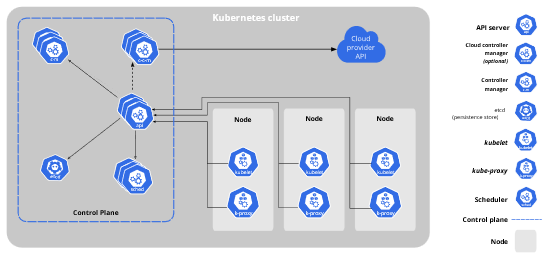
\includegraphics[width=0.9\textwidth]{resources/ch2/kube-1.png}
      \caption{Arsitektur Kubernetes \citep{kube-arch}}
      \label{KubeArch}
\end{figure}

Adapun komponen-komponen yang terdapat pada master node antara lain:
\begin{enumerate}
      \item Kube-apiserver adalah komponen dari master node yang mengekspos API Kubernetes. API Server adalah frontend dari worker node / control plane bagi Kubernetes.
      \item Etcd adalah komponen yang berfungsi sebagai penyimpan data yang konsisten dan higly-available dengan skema penyimpanan key-value.
      \item	Kube-scheduler berfungsi sebagai pengawas dan penjadwal bagi pod yang baru dibuat dan tugasnya adalah untuk menetapkan dimana node  bagi pod tersebut.
      \item	Kube-controller-manager adalah komponen yang berfungsi untuk menjalankan proses controller yaitu fungsi yang bertanggung jawab mengelola pod, worker node, dan mengatur tugas jika terjadi kegagalan pada proses pembuatan pod.
\end{enumerate}

Adapun komponen-komponen yang terdapat pada worker node antara lain:
\begin{enumerate}
      \item  Kubelet adalah komponen yang berfungsi sebagai agen di setiap node yang ada pada cluster dan bertugas untuk memastikan container yang berjalan pada pod.
      \item Kube-proxy adalah sebuah proxy jaringan yang berjalan di setiap node pada cluster dan mengimplementasikan konsep dari service Kubernetes.
      \item Container Runtime adalah sebuah perangkat lunak yang bertanggung jawab untuk menjalankan container. Kubernetes sendiri mendukung beberapa Container Runtime seperti Docker, containerd, CRI-O, dan semua jenis Runtime yang mengimplementasi Kubernetes CRI (Container Runtime Interface).
\end{enumerate}

\subsection{Pod}
Pod adalah unit terkecil yang dapat di deploy di dalam sebuah Kubernetes cluster.
Pod sendiri adalah sebuah abstraksi dari container yang di deploy di Kubernetes.
Jadi, ketika seorang pengguna ingin membuat sebuah aplikasi berbasis container di Kubernetes, pengguna tidak melakukan deploy container secara langsung melainkan melalui object Kubernetes yang bernama Pod.
Di dalam Pod sendiri bisa terdapat lebih dari satu buah container sekaligus sesuai dengan kebutuhan.
Contohnya ada jenis container yang disebut sebagai sidecar yang berfungsi sebagai secondary unit dari container utama yang ada di dalam Pod tersebut.
\subsection{Controller}
Kita bisa langsung membuat Pod di kubernetes lewat command line interface.
Namun jika kita membuat secara manual Pod, maka kita juga harus bertanggung jawab selama lifecycle dari Pod tersebut.
Masalah timbul ketika kita ingin membuat beberapa Pod yang sama sekaligus, maka akan menjadi suatu tugas yang tidak mudah untuk mengatur Pod-Pod tersebut.
Dari permasalahan itulah, ada sebuah konsep di Kubernetes yang disebut dengan Controller.

Controller adalah sebuah abstraksi di atas Pod yang bertugas untuk mengelola Pod secara otomatis dengan memanfaatkan komponen di dalam Pod yang bernama Container Probes.
Container Probes akan berfungsi untuk melakukan pengecekan apakah container yang berada di Pod berjalan dengan baik.
Jika Container Probes memberi tahu Controller bahwa container tidak berjalan dengan baik, maka Controller akan melakukan reset pada container tersebut.

Pada implementasinya, Kubernetes memiliki dua jenis implementasi dari Controller yaitu ReplicaSet dan DaemonSet.

\subsection{ReplicaSet}
ReplicaSet adalah jenis Controller yang bertanggung jawab untuk mengelola kebutuhan Pod sesuai state yang dispesifikkan oleh pengguna.
Cara ReplicaSet melakukan monitor pada Pod adalah melalui label yang telah ditetapkan ke sebuah Pod.
Jika label tersebut dengan selector yang terdapat pada ReplicaSet maka Pod akan masuk ke pengawasan dari ReplicaSet.
ReplicaSet akan mencocokkan keadaan Pod dengan spesifikasi yang diberikan oleh pengguna sehingga ketika ReplicaSet melihat bahwa Pod tidak sesuai dengan spesifikasi, contohnya banyaknya Pod tidak sesuai, ataupun satu node mati sehingga Pod yang ada di dalamnya terdampak, maka ReplicaSet akan menyesuaikan kondisi Pod tersebut.

\subsection{DaemonSet}
DaemonSet adalah jenis Controller yang memiliki fungsi untuk mengatur agar tepat ada satu Pod pada setiap node.
DaemonSet biasanya digunakan untuk mengelola Pod yang erat fungsinya dengan infrastruktur dari Kubernetes seperti mengatur jalannya operasi sistem, mengumpulkan log, atau memonitor resource di setiap node.

\subsection{Deployment}
Deployment adalah suatu abstraksi Controller di atas ReplicaSet yang tugasnya adalah melakukan deployment aplikasi Container di Kubernetes.
Deployment akan bekerja dengan mengatur ReplicaSet yang ada untuk mengatur pembaruan yang terjadi pada sebuah versi aplikasi Deployment.
Cara yang dilakukan oleh Deployment dalam mengatur versi aplikasi adalah dengan mengontrol ReplicaSet yang mengatur Pod.
Jika kita melakukan upgrade sebuah aplikasi pada Deployment, pertama kali Deployment akan menginstruksikan kepada ReplicaSet untuk mengurangi jumlah Pod yang diatur hingga nol.
Baru kemudian Deployment menginstruksikan kembali ReplicaSet untuk membuat Pod sebanyak spesifikasi.

Dengan fitur semacam itu, Deployment dapat memberikan fungsionalitas update tanpa adanya down time seperti melakukan rollback jika versi Deployment yang baru tidak sesuai yang diinginkan oleh pengguna.

\subsection{Service}
Fungsi networking adalah salah satu yang terpenting dalam sebuah sistem terdistribusi sebab suatu komponen perlu untuk berkomunikasi dengan komponen lainnya, dalam hal ini Pod.
Seperti yang sudah dipaparkan sebelumnya, Pod akan dikontrol oleh Controller, dalam hal ini adalah ReplicaSet melalui Deployment.
Dari sistem itu, ada kemungkinan bahwa Pod ynag berisi sebuah aplikasi container akan berubah sesuai yang dikehendaki oleh Controller-nya.
Jika kita melakukan komunikasi antar Pod langsung melalui IP address dari Pod tersebut, maka jika Pod tersebut hilang atau digantikan oleh Controller-nya maka IP address yang lama akan tidak bisa digunakan kembali.

Untuk menyelesaikan permasalahan tersebut, Kubernetes menggunakan sebuah layer abstraksi untuk Networking yang dinamakan Service.
Service akan menyediakan entry kepada sebuah Pod melalui Controller-nya, yaitu Deployment dan Service akan menyediakan IP address dan juga DNS entry yang tetap sehingga ketika Pod di dalam Deployment tersebut berubah, Pod akan tetap bisa diakses melalui Service.

Untuk memudahkan discovery dari sebuah Service, kubernetes memiliki sistem DNS nya sendiri yang diatur melalui master node.
Cara mengakses nya secara standar adalah jika pada sebuah Namespace yang sama, komponen Kubernetes yang lain dapat mengakses Service dan port nya langsung dengan format nama service itu sendiri.
Namun jika sebuah komponen Kubernetes lainnya mengakses Service tersebut dari luar Namespace tempat Service di deploy, maka cara pengaksesannya mengikuti format seperti berikut: \textit{[nama service].[namespace].svc.cluster.local}.

Dalam mengakomodasikan kebutuhan networking di Kubernetes, Service sendiri memiliki beberapa jenis yang dapat digunakan untuk berbagai usecase yang berbeda.
Tipe-tipe Service tersebut adalah:
\begin{enumerate}
      \item ClusterIP \\
            ClusterIP adalah tipe default dari Service. Seperti namanya, ClusterIP akan berbentuk sebuah IP address yang hanya bisa diakses dari dalam cluster dengan DNS.
      \item NodePort \\
            Dengan tipe Service ini, Kubernetes akan membuat sebuah port yang sama pada semua node yang dapat diakses dari luar cluster.
      \item LoadBalancer \\
            Tipe LoadBalancer adalah tipe Service khusus yang dipergunakan untuk mengekspos Service ke luar cluster melalui sebuah layanan Load Balancer. Layan Load Balancer yang dapat dipergunakan sendiri bisa dipilih sesuai dengan dimana cluster Kubernetes dibuat. Jika cluster dibuat di salah satu penyedia jasa Cloud Computing, maka LoadBalancer akan menggunakan layanan Load Balancer dari Cloud Computing tersebut untuk mengekspos Service ke luar cluster.
\end{enumerate}

\section{Database \textit{time-series}}

\section{Pendekatan untuk melakukan \textit{Performance Regression Analysis}}
Pada Subbab ini, akan dibahas beberapa pendekatan dan algoritme yang dapat digunakan untuk melakukan analisis pada regresi kinerja aplikasi berbasis Microservice.
\label{ch2-algo}
%\subsubsection{Integrasi dengan \textit{workflow} \textit{alerting}}


\subsection{Analisiis hasil \textit{Trace} individual}
Melihat hasil \textit{trace} individu adalah salah satu cara paling sederhana dalam memanfaatkan \textit{distributed tracing} sebagai bagian dari respon terhadap insiden dan analisis akar masalah \citep{parker2020distributed}. Hasil \textit{trace} individual dapat berguna terutama ketika kesalahan mudah diidentifikasi, seperti contohnya ada perubahan yang mengakibatkan kerusakan pada sebuah \textit{service}. Hal tersebut berarti semua \textit{request}, atau sebagian besar, gagal dalam eksekusinya, sehingga mudah untuk mengidentifikasi satu \textit{request} tersebut.

Risiko dari hanya menggunakan hasil \textit{trace} individual adalah karena perubahan dalam \textit{service} berjalan dengan cepat, akan sangat mungkin untuk menggeneralisir sebuah hasil \textit{trace} individual dan menyimpulkan penyebab yang salah dari sebuah insiden. 


%\subsubsection{Analisis sampel bias}


\subsection{Respons secara \textit{real-time}}
\label{approach-realtime}


\subsection{Analisis Kumulatif}
\label{approach-cumulative}

Salah satu cara untuk mengetahui kondisi metrik dari suatu sistem adalah dengan menggunakan histogram. Histogram sendiri adalah sebuah grafik yang menunjukkan perbandingan antara frekuensi kemunculan pada sumbu y dan metrik pada sumbu x. Artinya dengan histogram dapat ditunjukkan kondisi metrik dalam suatu sistem terdistribusi lewat tangkapan \textit{trace} secara keseluruhan. Salah satu metrik yang umum digunakan adalah latensi.

\begin{figure}[htb]
	\centering
	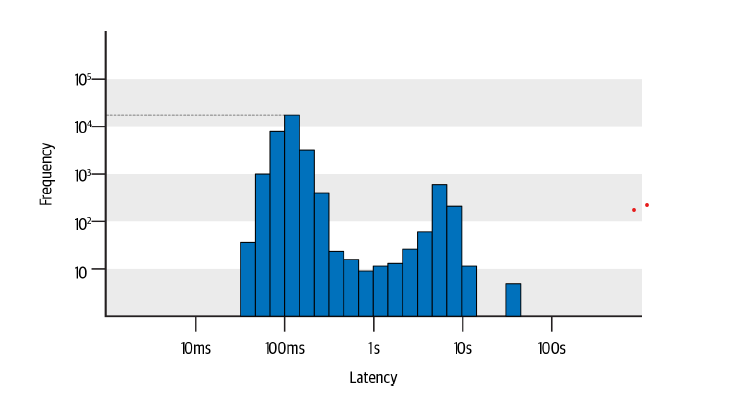
\includegraphics[width=1\textwidth]{resources/ch3/histogram-og.png}
	\caption{Contoh Histogram \citep{parker2020distributed}}
	\label{histogram}
\end{figure}

Ada beberapa teknik statistik yang dapat digunakan untuk mengetahui apakah dua buah sampel diambil dari sebuah distribusi yang sama. Salah satu teknik yang dapat digunakan adalah statistik Kolmogorov-Smirnov (K-S). Statistik K-S menghitung perbedaan dua buah distribusi sebagai sebuah bilangan skalar \citep{kolmogorov_1951}. Untuk mendapatkan distribusi tersebut, data yang berasal dari histogram akan terlebih dahulu diubah sebagai fungsi dengan fungsi distribusi kumulatif atau \textit{cumulative distribution function} (CDF). Ada dua perbedaan utama antara histogram dengan CDF. Pertama seperti namanya, CDF akan mengakumulasikan perhitungan, sehingga setiap titik pada CDF merupakan penjumlahan dari semua titik yang ada pada histogram di sebelah kiri. Kedua, sumbu y pada CDF dinormalisasi sehingga nilainya akan berkisar antara nol hingga satu. 

Gambar \ref{ks-example} menunjukkan dua buah CDF. Statistik K-S didapatkan dengan mencari jarak vertikal terjauh antara dua CDF seperti yang ditunjukkan oleh panah. Semakin besar jarak menunjukkan semakin mungkin bahwa dua buah CDF merupakan dua distribusi yang berbeda sehingga dapat menjadi indikasi bahwa terdapat perubahan pada kinerja. 

\begin{figure}[htb]
	\centering
	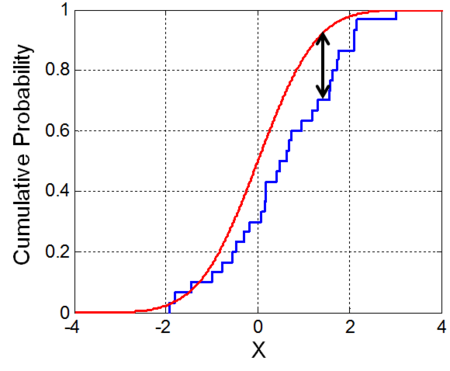
\includegraphics[width=0.6\textwidth]{resources/ch3/ks.png}
	\caption{CDF dari dua buah sampel, panah menunjukkan nilai statistik Kolmogorov-Smirnov \citep{wiki:ks-test}}
	\label{ks-example}
\end{figure}
%\subsection{Menentukan \textit{Critical Path}}b
%\label{approach-cp}
%Dalam setiap sistem terdistribusi yang cukup kompleks, selalu terdapat 

\subsection{Analisis Agregasi dan Korelasi}
\label{approach-corr}

Langkah pertama dalam menggunakan pendekatan ini adalah dengan membagi hasil \textit{trace} menjadi dua kelompok sampel, kedua jenis sampel ini akan menjadi basis bagi semua perbandingan kedepannya. Dengan asumsi regresi sudah diketahui terjadi, sampel bagian pertama harus berasal dari regresi itu sendiri. Hal tersebut mudah didapatkan jika regresi sedang terjadi sekarang. Jika regresi juga terjadi pada sebagian besar dari \textit{request}, maka sampel dari \textit{request} tersebut juga dapat menjadi penting. 

Bagian sampel kedua harus berasal dari kinerja \textit{baseline}. Hal tersebut dapat berasal dari sekumpulan \textit{trace} sebelum regeresi terjadi, mungkin dari satu jam, satu hari, atau bahkan satu minggu sebelumnya; artinya adalah pertama kali sekali, sistem \textit{tracing} harus memiliki terlebih dahulu catatan mengenai kinerja \textit{baseline} dari aplikasi. Catatan kinerja \textit{baseline} dapat diperoleh dari siklus penggunaan aplikasi oleh pengguna. Penggunaan alat visualisasi seperti histogram dapat dilakukan untuk mengidentifikasi sampel mana yang dapat menjadi representasi \textit{baseline} dari aplikasi.

Setelah dimiliki dua kelompok sampel (misal sampel A dan B) dan juga sekelompok fitur, analisis dilakukan dengan melihat setiap fitur dan mengajukan pertanyaan "Apa kemungkinan fitur tersebut ada pada sampel A tetapi tidak ada di sampel B?". Pertanyaan tersebut akan menghasilkan "koefisien korelasi" bagi setiap fitur. Koefisien yang bernilai 1.0 berarti sebuah fitur ada pada setiap \textit{trace} pada sampel A dan tidak pernah ada pada sebuah \textit{trace} di sampel B, sementara koefisien -1.0 berarti sebuah fitur yang ada pada setiap \textit{trace} di sampel B dan tidak pernah ada pada \textit{trace} di sampel A. Sebuah koefisien 0.0 berarti fitur tersebut secara seimbang dapat ada pada kedua sampel. Semakin dekat hasil ke 1.0 atau -1.0 sebuah koefisien korelasi, semakin mungkin sebuah fitur dapat menjelaskan perbedaan antara kedua sampel.

Metrik-metrik seperti \textit{latency}, \textit{error}, \textit{tag}, dan metadata lainnya dapat menjadi fitur yang berharga dari \textit{trace} yang dapat digunakan untuk memahami perubahan apa yang telah terjadi. Salah satu keunggulan dari penggunaan \textit{distributed tracing} adalah dapat menempatkan perubahan kinerja dalam konteks apa yang terjadi pada alur keberjalanan aplikasi. Ketika menentukan atribut apa dari \textit{trace} mana saja yang akan digunakan sebagai bagian dari analisis korelasi, harus diingat bahwa atribut tersebut haruslah berasal dari setiap \textit{span} pada \textit{trace} yang ada, bukan hanya yang terkait dengan sebuah \textit{service} tertentu.

Sebagai contoh, andaikan telah terjadi peningkatan \textit{latency} pada \textit{service} yang ada dan sebagai tindakannya kita membandingkan sampel \textit{trace} yang terjadi pada lima menit terakhir dengan sampel \textit{trace} yang terjadi pada satu jam yang lalu. Tabel \ref{corr-tab-1} menunjukkan sampel kecil dari fitur yang dapat diidentifikasi oleh analisis ini.

\begin{small}
	\begin{longtable}{ | p{10cm} | p{2cm} | }
			\caption{Contoh analisis korelasi}
			\label{corr-tab-1}                                                           
			\\ \hline
			\centering\bfseries{Fitur} & \centering\bfseries{Koefisien Korelasi} \tabularnewline \hline
			\endfirsthead
%			\hline
			\textbf{service}: inventory, \textbf{service.version}: 1.14.2 & 0.65 \\ \hline
			\textbf{runinfo.host}: vm73 & 0.41 \\ \hline
			\textbf{service}: inventory, \textbf{service.version}: 1.14.1 &  $\num{-0.65}$ \\ \hline
		\end{longtable}
\end{small}







\section{Penelitian Terkait}

%\subsection{Analisis Terotomasi dari \textit{Distributed Tracing}}
\subsection{Automated Analysis of Distributed Tracing}

\subsection{A Real-time Trace-level Root-cause Diagnosis System in Alibaba Datacenters}


\subsection{Dapper}

Dapper merupakan salah satu pionir teknologi \textit{distributed tracing} yang pertama kali dibuat oleh Google \citep{dapper-paper}. Dapper pertama kali dibuat untuk menyelesaikan permasalahan 

\subsection{Zipkin}

\subsection{Inkle}


%\chapter{Analisis Masalah dan Perancangan Solusi \textit{Performance Regression Analysis} menggunakan \textit{distributed tracing}}
\chapter{Analisis Masalah dan Perancangan Solusi}
%Pada bab ini diuraikan analisis persoalan pengumpulan data pada \textit{spreadsheet} yang telah diuraikan pada Bab I. Hasil dari bab ini digunakan untuk merancang kakas yang akan diimplementasikan seperti yang dijelaskan pada Bab IV.
%Berdasarkan 


\section{Analisis Masalah}

Seiring dengan meningkatnya kompleksitas dari aplikasi Microservice, seperti dengan meningkatnya jumlah service dan keterhubungan antar service yang ada di dalamnya, akan meningkat juga kompleksitas untuk melakukan \textit{monitoring} terhadap kinerja pada keseluruhan aplikasi Microservice. Salah satu isu penting terkait dengan kinerja adalah regresi atau penurunan terhadap kinerja. Kebutuhan untuk dengan segera menentukan penyebab utama dari regresi pada sistem menjadi penting apabila regresi terjadi pada lingkungan produksi yang langsung melayani \textit{request} dari pelanggan, sehingga apabila tidak diatasi dengan segera akan berdampak langsung terhadap pengalaman pengguna dalam menggunakan aplikasi. 

Terdapat dua pendekatan yang dapat dilakukan untuk mengatasi permasalahan regresi kinerja \citep{regression-detection}, yaitu:
\begin{enumerate}
	\item Deteksi regresi dilakukan setelah aplikasi selesai dikembangkan dan di-\textit{deploy} pada lingkungan terdedikasi
	\item Deteksi regresi dilakukan sebelum aplikasi selesai dikembangkan dan di-\textit{deploy} dan melakukan studi terhadap perubahan yang dihasilkan pada \textit{source code}
\end{enumerate}  

Mengingat sifat dari Microservice yang terdistribusi, akan menjadi sulit bagi \textit{developer} jika pendeteksian regresi dilakukan dengan pendekatan individual pada masing-masing service yang ada terlebih ketika jumlah service yang ada sudah sangat banyak dan hubungan interdependensi antar service menjadi rumit. Oleh karena itu, untuk mengatasi regresi kinerja pada aplikasi berbasis Microservice, dibutuhkanlah pendekatan yang tidak mengharuskan \textit{developer} untuk melakukan pencarian sumber masalah pada masing-masing service secara individu. Sehingga pada kasus deteksi dan analisis regresi kinerja aplikasi berbasis Microservice, pendekatan pertama lebih cocok untuk digunakan.

Salah satu teknologi yang dapat digunakan untuk melakukan \textit{monitoring} dan analisis regresi pada sebuah sistem terdistribusi seperti Microservice adalah \textit{distributed tracing}. Dengan bantuan mekanisme \textit{span} dari \textit{trace}, metrik-metrik kinerja dalam aplikasi berbasis Microservice dapat dilacak secara menyeluruh. Dalam kasus penggunaan seperti yang telah disebutkan sebelumnya, \textit{distributed tracing} cocok untuk digunakan dalam melakukan analisis regresi kinerja atau \textit{Performance Regression Analysis} dalam sebuah aplikasi berbasis Microservice sebab \textit{developer} tidak perlu menganalisis satu per satu \textit{service} yang ada terutama setelah \textit{service} sudah di-\textit{deploy}.

%Salah satu teknologi yang dapat menyediakan \textit{developer} kakas untuk melakukan \textit{monitoring} sebuah sistem terdistribusi secara keseluruhan adalah \textit{distributed tracing}. Dengan memanfaat

Oleh karena itu, dapat dirumuskan alur kerja yang harus dilakukan oleh sistem \textit{Performance Regression Analysis} (PRA) sebagai berikut:
\begin{enumerate}
	\item Sistem harus dapat mendeteksi ketika terjadi regresi pada aplikasi berbasis Microservice
	\item Sistem harus dapat menentukan sumber atau akar permasalahan dari regresi setelah terdeteksi
\end{enumerate}

%Untuk dapat melakukan 

%Adapun, langkah-langkah berikut dapat dilakukan untuk melakukan analisis penyebab regresi kinerja pada Microservice \citep{parker2020distributed}:
%\begin{enumerate}
%	\item Tentukan \textit{baseline} atau pengukuran dasar dari beberapa kinerja service
%	\item Ten
%\end{enumerate}

Sudah terdapat beberapa pendekatan yang dapat digunakan untuk melakukan analisis regresi seperti yang ada pada subbab \ref{ch2-algo}. Melihat kebutuhan dari sistem PRA di atas, dari beberapa pendekatan yang ada pada subbab tersebut, penulis menilai ada dua pendekatan yang dapat digunakan yaitu pendekatan Analisis Kumulatif pada \ref{approach-cumulative} dan pendekatan Analisis Agregasi dan Korelasi pada \ref{approach-corr}. Analisis Kumulatif dapat digunakan untuk menentukan apakah telah terjadi regresi pada aplikasi dengan melakukan perbandingan antara CDF \textit{baseline} dengan CDF dari aplikasi yang sedang berjalan. Ketika didapatkan statistik K-S yang melebihi \textit{threshold}, sistem PRA akan melakukan analisis akar permasalahan dengan metode Analisis Agregasi dan Korelasi untuk mendapatkan penyebab dari regresi melalui analisis \textit{crtical path} pada \textit{service} yang terdeteksi memiliki koefisien korelasi tinggi. Penghitungan koefisien korelasi dapat dilakukan dengan menghitung koefisien korelasi antara hasil \textit{trace} ketika terdeteksi regresi dengan hasil \textit{trace} dari \textit{baseline}.

Gambar \ref{alur-pra} menggambarkan fase yang akan dilakukan oleh sistem PRA. Secara umum, akan terdapat dua fase yang akan dilakukan yaitu fase \textit{baseline loading phase} dan fase \textit{realtime analysis phase}. Fase pertama yaitu \textit{loading} akan mencari data dari aktivitas aplikasi yang bersifat stabil yang dapat digunakan sebagai \textit{baseline} atau acuan bagi analisis yang akan dilakukan pada tahap selanjutnya. Fase ini akan menghasilkan dua buah artifak yaitu fungsi \textit{cumulative distribution function} (CDF) dari histogram hasil \textit{trace} dan juga data operasi yang terjadi pada \textit{critical path} semua \textit{span} beserta nilai \textit{latency}-nya yang akan disimpan sebagai pasangan \textit{key-value}. Fase berikutnya adalah fase analis secara \textit{realtime} yang akan membandingkan hasil transformasi CDF histogram \textit{span} yang sedang berlangsung sekarang dengan CDF \textit{baseline} hasil fase sebelumnya. Perbandingan tersebut akan dilakukan dalam periode tertentu. Untuk perancangan awal, periode waktu yang digunakan adalah selama 10 menit sekali. Perbandingan dari kedua CDF tadi akan menghasilkan statistik Kolmogorov-Smirnov (K-S). Jika statistik K-S yang dihasilkan melebihi batas \textit{threshold}, maka dapat disimpulkan bahwa terjadi regresi pada periode \textit{capture} histogram tersebut. 

\begin{figure}[htb]
	\centering
	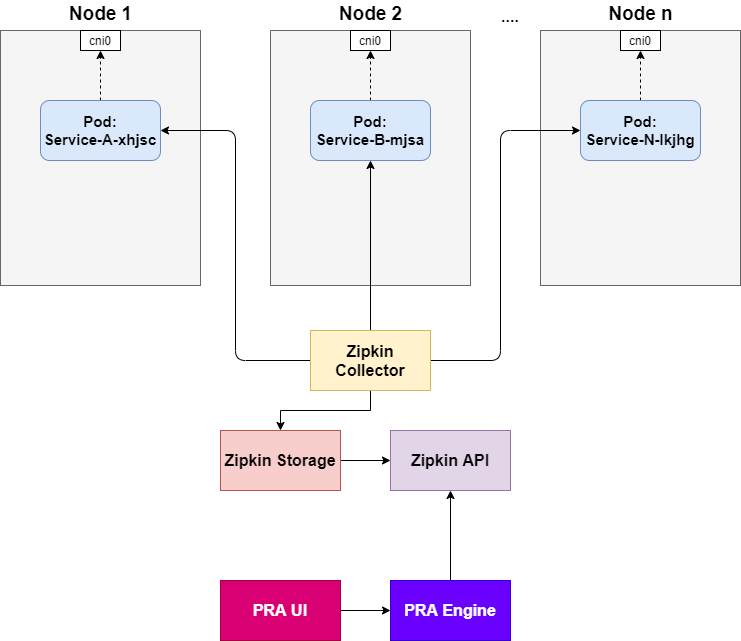
\includegraphics[width=1\textwidth]{resources/ch3/alur.png}
	\caption{Alur sistem \textit{Performance Regression Analysis}}
	\label{alur-pra}
\end{figure}

%Melihat kebutuhan untuk melakukan deteksi regresi secara terdistribusi pada Microservice, penulis menilai bahwa \textit{distributed tracing} dapat digunakan sebagai solusi untuk menyelesaikan masalah tersebut. Beberapa 


%ketika terjadi penurunan pada kinerja ataupun terdapat \textit{error} yang diakibatkan oleh suatu service tertentu.
%
%
%Regresi dalam sebuah sistem terdistribusi dapat diakibatkan oleh beberapa hal, contohnya adalah 
%\section{Analisis Alternatif Solusi} %Ngebandingin 

\section{Rancangan Solusi}

\subsection{Desain \textit{Payload}}

\subsection{Aristektur Solusi}

%\section{Rancangan Pengukuran \textit{Overhead}} % Di Bab 4

 \section{Jadwal Pelaksanaan}
 \newsavebox\mybox
 \begin{lrbox}{\mybox}
	     \begin{ganttchart}[
		     vgrid={*{6}{draw=none}, dotted},
		     x unit=.05cm,
		     y unit title=.6cm,
		     y unit chart=.6cm,
		     time slot format=isodate,
		     time slot format/start date=2016-09-01]{2021-09-01}{2022-04-30}
		     \ganttset{bar height=.6}
		     \gantttitlecalendar{year, month} \\
		     \ganttbar[bar/.append style={fill=blue}]{Studi Literatur}{2021-09-01}{2021-11-30}\\
		     \ganttbar[bar/.append style={fill=blue}]{Analisis Masalah}{2021-10-01}{2021-11-15}\\
		     \ganttbar[bar/.append style={fill=blue}]{Perancangan Solusi}{2021-11-01}{2021-12-15}\\
		     \ganttbar[bar/.append style={fill=blue}]{Implementasi}{2021-12-15}{2022-03-01}\\
		     \ganttbar[bar/.append style={fill=blue}]{Pengujian dan Analisis Hasil}{2022-02-01}{2022-04-30}
		     \end{ganttchart}
	 \end{lrbox}

 Pengerjaan tugas akhir ini direncanakan mulai pada September 2021 sampai April 2022. Pelaksanaan tugas akhir ini dibagi menjadi 5 tahap yang dapat dipetakan kepada metodologi pengerjaan sebagai berikut,
 \begin{enumerate}
	     \item Tahap 1: Studi Literatur
	     \item Tahap 2: Analisis Masalah
	     \item Tahap 3: Perancangan Solusi
	     \item Tahap 4: Implementasi
	     \item Tahap 5: Pengujian dan Analisis Hasil
	 \end{enumerate}
 Jadwal pelaksanaan tugas akhir berdasarkan metodologi pengerjaan tugas akhir dapat dilihat pada Tabel \ref{Gantt-Chart} dibawah ini.
 \begin{table}[htb]
	 \centering
	 \caption{Gantt Chart jadwal pelaksanaan tugas akhir}
	 \label{Gantt-Chart}
	 \tikz{
		   \node[inner sep=0pt,outer sep=0pt] (gantt)
		   {\begin{tabular}{c}
				     \toprule
				     \resizebox{\textwidth}{!}{\usebox\mybox} \\
				     \bottomrule
				    \end{tabular}%
			    };
		 }   
	 \end{table}

% Pada masa sebelum adopsi arsitektur Microservice dan kebanyakan dari aplikasi masih menggunakan arsitektur Monolith, proses seperti \textit{debugging} adalah hal yang sederhana sebab jika terdapat suatu \textit{error} akan mudah untuk ditelusuri dari mana asal \textit{error} tersebut sebab hanya ada satu aplikasi yang digunakan. Hal tersebut tidak berlaku jika aplikasi menggunakan model Sistem Terdistribusi, salah satu contohnya adalah Microservice. Sifat dari Microservice yang melakukan \textit{decoupling} aplikasi menjadi bagian yang lebih kecil membuat proses \textit{debugging} menjadi tidak mudah sebab untuk mencari penyebab \textit{error} aplikasi yang terdistribusi, kita harus mengetahui terlebih dahulu sumber dari \textit{error} tersebut. Kompleksitas akan bertambah dalam proses debugging jika ternyata ditemukan bahwa sautu \textit{error} pada sebuah \textit{service} bukanlah akar atau penyebab utama dari \textit{error} tersebut melainkan suatu \textit{service} lainnya. Kompleksitas akan bertambah jika metode \textit{debugging} yang digunakan mengharuskan \textit{developer} yang menangani \textit{error} tersebut harus menelusuri satu per satu \textit{service} yang terdampak sampai menemukan akar dari masalahnya. Dari masalah tersebutlah timbul suatu kebutuhan untuk mendapatkan gambaran mengenai \textit{state} sebuah Sistem Terdistribusi ataupun yang disebut juga dengan \textit{observability}.
% 
% 
% 
% Dengan bantuan dari \textit{trace} atau yang disebut \textit{distributed tracing}, \textit{developer} bisa mendapatkan suatu gambaran dari masing-masing \textit{request} yang terjadi pada sebuah \textit{resource} atau komponen yang berinteraksi dengan komponen lainnya dalam sebuah Sistem Terdistribusi seperti \textit{node}, \textit{service}, \textit{network}, ataupun \textit{mutex}. Ide dasar dari \textit{tracing} seperti yang sudah dijelaskan pada \ref{bab2-dtracing} adalah dengan mengidentifikasi sebuah titik spesifik, dapat jadi sebuah pemanggilan \textit{remote procedure call} (RPC), dalam sebuah aplikasi, \textit{library}, ataupun \textit{middleware} dalam jalur sebuah \textit{request} yang merepresentasikan kedua hal berikut:
% \begin{enumerate}
% \item \textit{Fork} pada eksekusi di level Sistem Operasi
% \item Sebuah lompatan atau akses horizontal ke luar melalui jaringan
%\end{enumerate}
%
%Data hasil \textit{trace} yang berisi kumpulan \textit{span} kemudian direpresentasikan sebagai \textit{directed acylic graph} (DAG), yang mana \textit{edge} antar graf dalam DAG yang disebut dengan \textit{reference} merepresentasikan hubungan atau kausalitas antar komponen dalam sebuah \textit{cluster} sistem terdistribusi yang terjadi pada \textit{request}. 
%
%
%
%Dengan meningkatkan performa \textit{baseline} pada sistem, para \textit{developer} berharap dapat meningkatkan kepuasan pelanggan, menurunkan biaya infrastruktur, ataupun keduanya. Untuk aplikasi yang langsung melayani pelanggan, performa seringkali berarti \textit{latency} dari \textit{request}. Proses optimisasi seperti ini biasanya adalah proses bertahap yang membutuhkan waktu.
%
%Kakas yang digunakan untuk membantu mencapai \textit{observability} penting untuk meningkatkan performa \textit{baseline} dengan pertama kali mengukur performa awal yang menjadi \textit{baseline} pengukuran dan digunakan untuk mengarahkan para \textit{developer} agar dapat mencari bagian mana dari aplikasi yang dapat ditingkatkan performanya. Dengan aplikasi yang menggunakan arsitektur Monolith, para \textit{developer} dapat dengan mudah melakukan \textit{profiling} proses mana saja yang dapat ditingkatkan penggunaan \textit{resource}-nya seperti CPU ataupun Memory. Namun dengan penggunaan arsitektur Microservice yang berbasis sistem terdistribusi, terkadang sulit untuk mengetahui \textit{service} manakah yang tepatnya perlu ditingkatkan penggunaan \textit{resource}-nya, sehingga penggunaan \textit{distributed tracing} akan sangat membantu untuk meningkatkan performa \textit{baseline} dari sebuah sistem terdistribusi.
%
%Berbeda dengan tujuan untuk meningkatkan performa \textit{baseline}, tujuan lainnya yaitu untuk mengembalikan performa \textit{baseline} bukanlah suatu hal yang dapat begitu saja direncanakan. Regresi dalam performa dapat muncul tiba-tiba seperti terjadinya \textit{outtage} atau pemberhentian tiba-tiba dari sebuah \textit{cluster} sistem terdistribusi. Melihat sifat dari sistem terdistribusi, mencari penyebab utama dari sebuah \textit{outtage} bukanlah sebuah hal yang mudah terlebih jika ada ratusan bahkan ribuan \textit{node} yang terdapat pada \textit{cluster} dan masing-masing \textit{node} saling terhubung dengan yang lainnya. Jika hal semacam tersebut terjadi dalam lingkungan aplikasi \textit{production} maka dampaknya akan terasa langsung oleh pelanggan dan dalam jangka panjang dapat menimbulkan kerugian material. Oleh karena itu, penting untuk segera mengetahui sumber atau akar dari suatu kejadian yang menyebabkan regresi pada performa sistem.
%
%Dari solusi \textit{distributed tracing} bersifat \textit{open source} yang tersedia saat ini, Zipkin dan Jaeger adalah dua solusi \textit{tracing} yang sudah menyediakan komponen instrumentasi, \textit{deployment}, dan \textit{value delivery} dalam bentuk \textit{application programming interface} (API) dan \textit{user interface} secara \textit{default}. Berikut adalah tabel perbandingan dari fitur \textit{user interface} web Zipkin dan Jaeger.
%
%
%\begin{small}
%	\begin{longtable}{ | p{3.75cm} | p{5.5cm} | p{5.5cm} | }
%		\caption{Deskripsi Perbandingan fitur Zipkin dan Jaeger}
%		\label{jzipkin-comparison}                                                                                                                \\ \hline
%		 & \centering\bfseries{Jaeger \citep{jaeger}} & \centering\bfseries{Zipkin \citep{zipkin}} \tabularnewline \hline
%		\endfirsthead
%		\bfseries{Deskripsi Singkat} & Dirilis sebagai kakas \textit{open-source} oleh Uber Technologies. Jaeger digunakan untuk melakukan \textit{monitoring} dan \textit{troubleshoot} dari sistem terdistribusi yang berbasis Microservice & Membantu mengumpulkan data bersifat temporal yang dibutuhkan untuk melakukan \textit{troubleshoot} permasalahn \textit{latency} pada aplikasi Microservice. Zipkin mengatur pengoleksian dan juga pencarian data. Desain dari Zipkin dibuat berdasarkan \textit{paper} dari Daper \citep{dapper-paper}\\ \hline
%		\bfseries{Kelebihan} &  \textit{Open-source}; 
%		Siap digunakan dengan Docker; Antarmuka dari \textit{collector} cocok digunakan dengan protokol milik Zipkin; Tingkat \textit{sampling} yang bersifat dinamis; Memiliki antarmuka berbasis Web &  \textit{Open-source}; 
%		Siap digunakan dengan Docker; Dapat menggunakan teknologi transport bagi \textit{span} yang berbeda-beda (HTTP, Kafka, Scribe, AMQP); Memiliki antar muka berbasis Web  \\ \hline
%		\bfseries{Kekurangan} & Hanya mendukung dua teknologi transport untuk \textit{span} (Thrift dan HTTP) & Tingkat \textit{sampling} yang bersifat \textit{fixed} \\ \hline
%		\bfseries{Jenis Analisis tersedia} & Visualisasi graf dependensi; Perbandingan hasil \textit{trace} & Visualisasi graf dependensi \\ \hline
%	\end{longtable}
%\end{small}
%
%Dari pemaparan mengenai kedua tujuan dari \textit{observability} di atas dan berdasarkan studi terhadap solusi \textit{open-source} yang sudah ada, penulis menyimpulkan bahwa ada dua hal yang dapat dibuat dengan menggunakan \textit{distributed tracing} untuk mencapai kedua tujuan utama dari \textit{observability}:
%\begin{enumerate}
%	\item Membuat Service Map untuk mencapai tujuan pertama yaitu meningkatkan performa baseline
%	\item Membuat perangkat untuk melakukan Root Cause Analysis (RCA) untuk mencapai tujuan kedua yaitu mengembalikan performa baseline ketika terjadi regresi pada sistem
%\end{enumerate}
%
%Service Map merupakan visualisasi dari sebuah sistem Microservice yang melakukan dekomposisi pada semua komponen \textit{service} dan menggambarkan dependensi yang terlihat antar \textit{service} tersebut secara \textit{real-time}, sehingga \textit{developer} dapat mengidentifikasi \textit{bottleneck} yang ada dan memahami bagaimana data mengalir dalam aristektur \citep{datadog-svcmap}. Untuk dapat membantu meningkatkan performa \textit{baseline}, sebuah Service Map harus dapat menyediakan informasi mengenai hubungan interdependensi antara \textit{service}, jumlah \textit{request} yang diterima oleh service per satuan waktu, dan ukuran performa pada \textit{service} tersebut dalam merespon \textit{service} lainnya. Ukuran performa yang dapat dijadikan \textit{baseline} antara lain adalah \textit{latency}, \textit{failure rate}, \textit{traffic rate}, dan saturasi, namun biasanya \textit{developer} hanya berfokus pada pengukuran \textit{latency} dan \textit{failure rate} \citep{parker2020distributed}.
%
%Selain digunakan untuk mendapatkan gambaran mengenai komponen yang ada pada suatu \textit{cluster} sistem terdistribusi, salah satu pendekatan yang dapat digunakan oleh Service Map untuk meningkatkan performa \textit{baseline}  disebut \textit{Correlation Analysis} \citep{parker2020distributed}. Untuk melakukan \textit{Correlation Analysis}, dibutuhkan tidak hanya satu tetapi dua sampel dari \textit{trace}. Satu sampel harus dapat merepresentasikan kelas \textit{trace} yang hendak dieliminasi atau setidaknya dikurangi jumlahnya, contohnya \textit{request} yang gagal atau lambat. Sampel jenis kedua harus dapat merepresentasikan komplemen dari sampel yang pertama, biasanya sekelompok \textit{request} yang cepat atau sukses. Selain dari dua kelompok sampel tadi, dibutuhkan juga sekelompok fitur yang dapat dicari korelasinya. Fitur-fitur yang dicari dalam sebuah sistem terdistribusi antara lain adalah \textit{service}, operasi, \textit{error}, dan \textit{tag} yang berasosiasi dengan \textit{span} yang membuat \textit{trace} tersebut. 
%
%Setelah dimiliki dua kelompok sampel (misal sampel A dan B) dan juga sekelompok fitur, analisis dilakukan dengan melihat setiap fitur dan mengajukan pertanyaan "Apa kemungkinan fitur tersebut ada pada sampel A tetapi tidak ada di sampel B?". Pertanyaan tersebut akan menghasilkan "koefisien korelasi" bagi setiap fitur. Koefisien yang bernilai 1.0 berarti sebuah fitur ada pada setiap \textit{trace} pada sampel A dan tidak pernah ada pada sebuah \textit{trace} di sampel B, sementara koefisien -1.0 berarti sebuah fitur yang ada pada setiap \textit{trace} di sampel B dan tidak pernah ada pada \textit{trace} di sampel A. Sebuah koefisien 0.0 berarti fitur tersebut secara seimbang dapat ada pada kedua sampel. Semakin dekat hasil ke 1.0 atau -1.0 sebuah koefisien korelasi, semakin mungkin sebuah fitur dapat menjelaskan perbedaan antara kedua sampel. 
%
%Di sisi lain, kakas untuk melakukan Root Cause Analysis dapat digunakan untuk memberikan petunjuk kepada \textit{developer} mengenai komponen mana dari Microservice yang mengalami regresi sehingga \textit{developer} dapat mengatasi permasalahan tersebut dengan segera. Salah satu pendekatan yang bisa dilakukan untuk mengembalikan performa adalah dengan pendekatan \textit{Aggregate and Correlation Root Cause Analysis} \citep{parker2020distributed}. Tidak jauh berbeda dengan pendekatan yang telah terlebih dahulu disebutkan pada Service Map, pendekatan ini menggunakan agregasi dari beberapa \textit{trace} untuk mendapatkan koefisien korelasi mengenai keadaan performa sebuah \textit{service}. 
%
%Adapun dari pemaparan di atas mengenai fitur analisis \textit{distributed tracing}, penulis menyimpulkan kebutuhan fungsional apa saja yang diperlukan pada pembuatan kakas visualisasi \textit{distributed tracing}:
%
%\begin{small}
%	\begin{longtable}{ | p{2cm} | p{10cm} | }
%		\caption{Kebutuhan Fungsional kakas visualisasi}
%		\label{fr-vis}                                                                                                                     \\ \hline
%		\centering\bfseries{ID} & \centering\bfseries{Deskripsi} \tabularnewline \hline
%		\endfirsthead
%		\hline
%		\centering\bfseries{ID} & \centering\bfseries{Deskripsi} \tabularnewline \hline
%		\endhead
%		FR-01 & Kakas dapt menampilkan hubungan interdependensi antara \textit{service} \\ \hline
%		FR-02 & Kakas dapat menampilkan pengukuran performa \textit{latency} pada setiap \textit{service} \\ \hline
%		FR-03 & Kakas dapat melakukan \textit{Correlation Analysis} untuk menentukan komponen mana dari Microservice yang dapat ditingkatkan performanya \\ \hline
%		FR-04 & Kakas dapat melakukan Root Cause Analysis (RCA) ketika terjadi sebuah regresi pada sistem dengan menggunakan pendekatan \textit{Aggregate and Correlation Root Cause Analysis} \\ \hline
%	\end{longtable}
%\end{small}






%Untuk mencapai kedua tujuan dari \textit{observability} tersebut, \textit{distributed tracing} dapat digunakan untuk menyediakan hal-hal berikut:
%\begin{enumerate}
%	\item 
%\end{enumerate}



%Seiring dengan meningkatnya penggunaan arsitektur, mengingkat pula kebutuhan bagi para \textit{developer} untuk dapat dengan segera mengetahui sumber dari permasalahan jika terjadi \textit{error} pada sistem.
%
%Dari pemaparan mengenai masih kurangnya kakas visualisasi \textit{tracing} yang bersifat \textit{open source}
%. Berdasarkan studi literatur mengenai \textit{observability} untuk Sistem Terdistribusi pada \ref{bab2-observability}, terdapat 

%Isu visualisasi 
%Overhead



%----------------------------------------------------------------%

% Daftar pustaka
% Bibliography to Daftar Pustaka
\renewcommand{\bibname}{Daftar Pustaka}
\clearpage
\phantomsection
\pagenumbering{roman}
\setcounter{page}{\thesavepage}
\bibliography{references}
\bibliographystyle{apalike}


\end{document}
